\documentclass[12pt, letterpaper]{article}
\usepackage[spanish]{babel}
\usepackage[utf8]{inputenc}
\usepackage{graphicx}
\usepackage{amssymb}
\graphicspath{{./imagenes/}}
\usepackage{xcolor}

%Paquetes para símbolos y entornos matematicos. En este documento se usa para poder usar el tag \begin{align} y \begin{align*} que permiten alinear expresiones matemáticas
\usepackage{amsmath}
\usepackage{amssymb}
%paquete que permite el uso de del argumento H al momento de insertar imágenes
\usepackage{float}

%comando para especificar el título del documento 
\title{Matemáticas para las Ciencias Aplicadas I}

%comando para especificar el autor del documento
\author{Pérez Romero Natalia Abigail}

%comando para especificar la fecha del documento
\date{\today}
%--------------Fin preámbulo--------------

%------------Inicio documento-------------
\begin{document}
%comando que genera el titulo con los datos especificados en el preámbulo
\maketitle
\textbf{Tarea VII. Ejercicios del libro Cálculo. Una variable de Thomas J.R, George B.}

\textbf{Ejercicios 4, 19, 21, 51 y 57  de  la sección 1.6 Funciones Trigonométricas}

\textbf{4.} Si una llanta de 1 m de diámetro se rueda hacia adelante 30 cm sobre el piso, ¿Qué angulo girará la llanta? Dé su respuesta en radianes (redondeando al décimo más cercano) y en grados (redondeando al grado más cercano).\\

La longitud de una circunferencia(perimetro) es  igual a $\pi$ * diametro. El perimetro de la llanta es igual a $1 * \pi$ que es $\pi$ m\\

\textbf{Fórmula de longitud de arco, con el ángulo en grados:}
Como una circunferencia es un arco con ángulo $360 ^{\circ}$, la longitud de un arco con ángulo $\alpha ^{\circ}$ en grados es
\begin{align*}
	L_{\alpha ^{\circ}}=  \frac{2 * \pi * r *  \alpha^{\circ}}{360^{ \circ}}
\end{align*}

\textbf{Fórmula de longitud de arco, con el ángulo en radianes:}
Si escribimos el ángulo $\alpha$ en radianes, la fórmula es
\begin{align*}
	L_{\alpha ^{\circ}}= \pi * \alpha^{\circ}
\end{align*}


En grados  

\begin{align*}
	L_{\alpha ^{\circ}}=  \frac{2 * \pi * r *  \alpha^{\circ}}{360^{ \circ}} \\
	30 cm =  \frac{2 * \pi * 0.5 *  \alpha^{\circ}}{360^{ \circ}}\\
	360 * 30 = 2 * \pi * 0.5 *  \alpha^{\circ}\\
	10800 = \pi * \alpha^{\circ}
\end{align*}




\textbf{Trace las gráficas de las funciones trigonométricas dadas, ¿Cuál es el periodo de cada función?}\\
\textbf{19} $\cos (x - \frac{\pi}{2})$

\begin{figure}[ht]
\centering
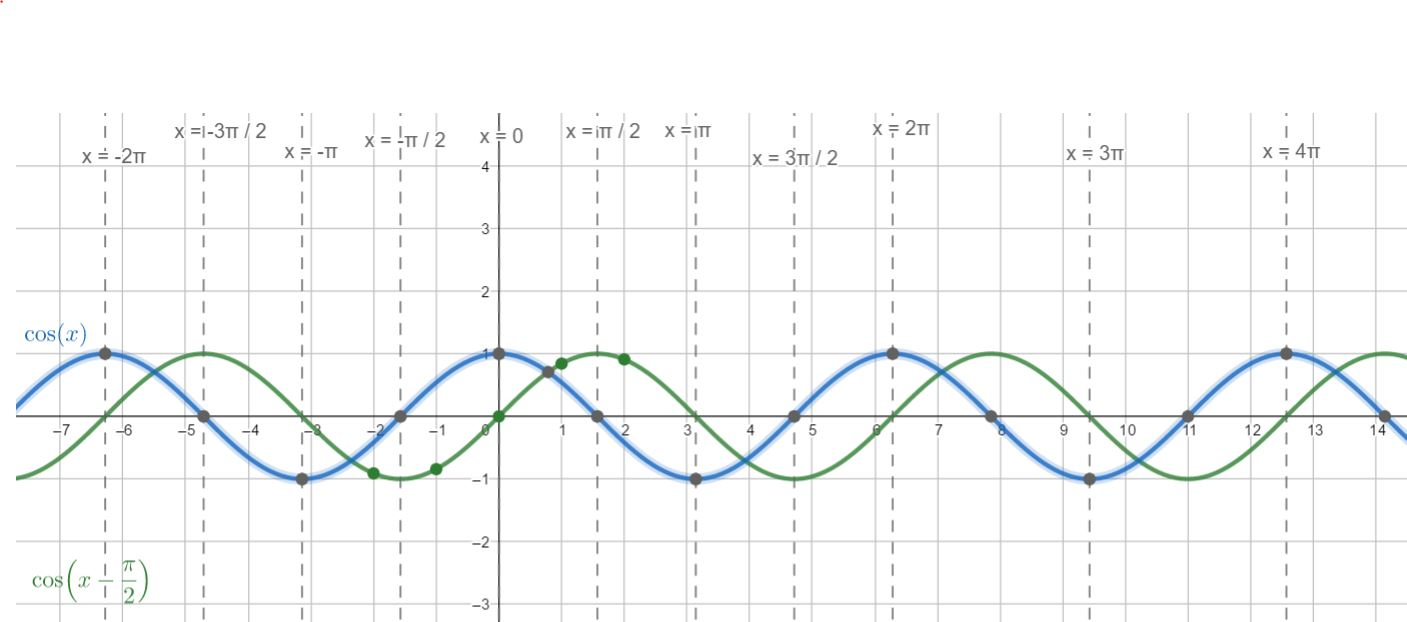
\includegraphics[width=40em]{t7dos}
\end{figure}

Recordando que podemos trasladar una función horizontalmente de está manera $y = f(x+h)$, si $h < 0$ el desplazamiento de la función se dará a la derecha $h$ unidades. Así que $\cos (x - \frac{\pi}{2})$ es la función $\cos (x)$ desplazada $\frac{\pi}{2}$ unidades  a la derecha. Por lo que  $\cos (x - \frac{\pi}{2})$ tiene el mismo periodo de $\cos (x)$

Podemos observar en la gráfica de la función $\cos(x)$ que cuando $x = 0, y = 1$, cuando $x=\pi, y= -1$, y cuando $x = 2\pi, y=1$, y esté patron se repite, los multiplos pares de $\pi$ valen 1 como cuando $x = 0$ por lo que se dice que la función $\cos (x)$ tiene un periodo de $2\pi$\\

Esto se debe a que al analizar la función en el círculo unitario $\cos (x) = \frac{CatetoAdyacente}{Hipotenusa} = \cos(x) = \pi$, ya que  $hipotenusa=1$, al recorrer el ciírculo modificando el valor del angulo $x$ tenemos que: cuando $x = 0, y=1$ porque el radio es 1,  cuando $x = \pi / 2, y = 0$ ,  cuando $x = \pi, y = -1$ debido a que $x$ se desplazo en sentido contrario a las manecillas del reloj, es decir, $x$ es un ángulo negativo; despues cuando $x=2\pi$ de nuevo $y=1$ y comienza otra vez el recorrido por el círculo.
\begin{figure}[ht]
\centering
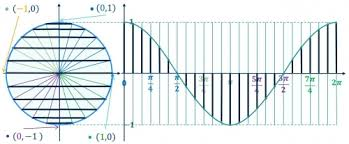
\includegraphics[width=30em]{t7tres}
\end{figure}

\newpage

\textbf{21} $\sen (x - \frac{\pi}{4}) + 1$

Recordando que podemos trasladar una función horizontalmente de está manera $y = f(x+h)$, si $h < 0$ el desplazamiento de la función se dará a la derecha $h$ unidades, también sabemos que podemos desplazar la gráfica hacia arriba sumandole una constante $k$. Así que $\sen (x - \frac{\pi}{4}) + 1$ es la función $\sen (x)$ desplazada $\frac{\pi}{4}$ unidades  a la derecha y una unidad hacia arriba. Por lo que $\sen (x - \frac{\pi}{4}) + 1$ tiene el mismo periodo $\sen (x)$

Podemos observar en la gráfica de la función $\sen$ que cuando $x = 0, y = 0$, cuando $x=\pi, y= 0$, y cuando $x = 2\pi, y= 0$, y esté patron se repite, los multiplos pares de $\pi$ valen 0 como cuando $x = 0$ por lo que se dice que la función $\cos (x)$ tiene un periodo de $2\pi$\\

\begin{figure}[ht]
\centering
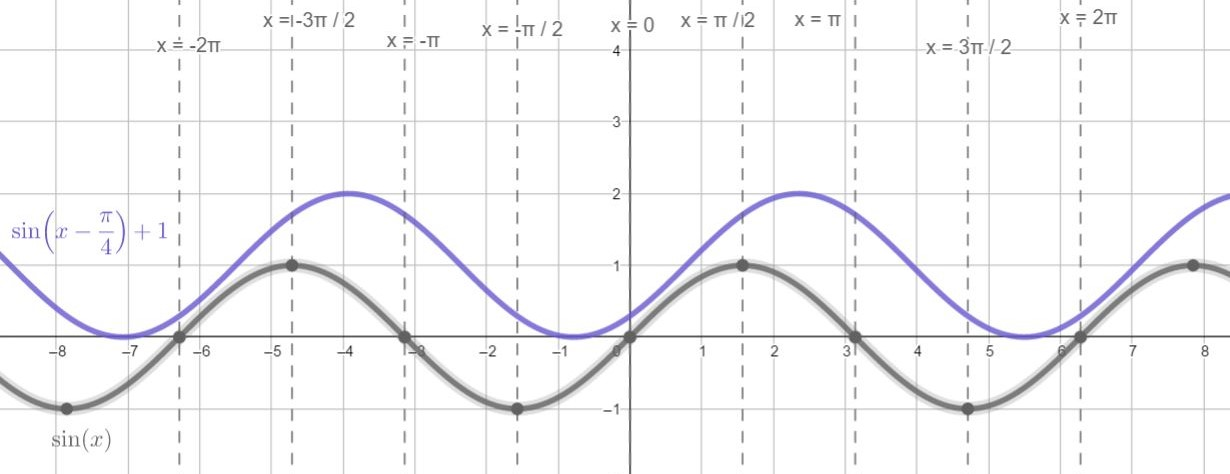
\includegraphics[width=40em]{t7cuatro}
\end{figure}


Esto se debe a que al analizar la función en el círculo unitario $\cos (x) = \frac{CatetoAdyacente}{Hipotenusa} = \cos(x) = \pi$, ya que  $hipotenusa=1$, al recorrer el ciírculo modificando el valor del angulo $x$ tenemos que: cuando $x = 0, y=1$ porque el radio es 1,  cuando $x = \pi / 2, y = 0$ ,  cuando $x = \pi, y = -1$ debido a que $x$ se desplazo en sentido contrario a las manecillas del reloj, es decir, $x$ es un ángulo negativo; despues cuando $x=2\pi$ de nuevo $y=1$ y comienza otra vez el recorrido por el círculo.
\begin{figure}[ht]
\centering
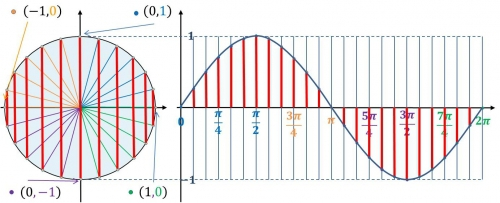
\includegraphics[width=30em]{t7cinco}
\end{figure}

\textbf{51. La fórmula de la tangente de una suma.} La forma estándar para la tangente de la suma de dos ángulos es

\begin{align*}
	tan (A + B) =  \frac{\tan A + \tan B}{1 - \tan A \tan B}
\end{align*}
Aplicando las identidades de senos y cosenos encuentre esta identidad trigonométrica para la tangente.

\textbf{57. La ley de los senos} afirma que si $a, b$ y $c$ son los lados opuestos a los ángulos $A, B$ y $C$ en un triángulo, entonces

\begin{align*}
 	\frac{\sen A}{a} =  \frac{\sen B}{b} = \frac{\sen C}{c}
\end{align*}

Use las siguientes figuras y, si lo requiere, la identidad $sen(\pi - \theta = \sen \theta$, para obtener la ley de senos.

\begin{figure}[ht]
\centering
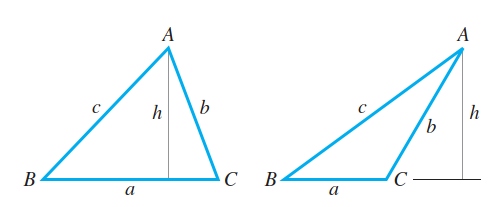
\includegraphics[width=20em]{t7uno}
\end{figure}


\end{document} 